\documentclass[10pt,a4paper]{article}
\usepackage[top=1.5cm, bottom=1.5cm, left=1.6cm, right=1.6cm, headheight=14pt, footskip=18pt]{geometry}
\usepackage[utf8]{inputenc}
\usepackage{amsmath,amsfonts,amssymb}
\usepackage{graphicx}
\usepackage{tikz}
\usepackage{circuitikz}
\usetikzlibrary{calc,patterns}
\usepackage[most]{tcolorbox}
\usepackage{enumitem}
\usepackage{fancyhdr}
\usepackage{booktabs}
\usepackage{tabularx}
\usepackage{colortbl}
\usepackage{hyperref}

% --- Palet Warna Resmi UNIB ---
\definecolor{unibblue}{RGB}{0, 32, 96}
\definecolor{unibgold}{RGB}{197, 160, 89}
\definecolor{unibgreen}{RGB}{34, 112, 60}
\definecolor{boxbg}{RGB}{248, 250, 253}
\definecolor{linegray}{RGB}{210, 215, 225}

% --- Pengaturan Header & Footer ---
\pagestyle{fancy}
\fancyhf{}
\lhead{\footnotesize\textbf{\color{unibblue}Universitas Bengkulu} \textbar\ Program Studi S1 Teknik Elektro}
\rhead{\footnotesize\color{gray}Persamaan Diferensial (Genap 2026)}
\lfoot{\footnotesize\color{gray}LKM OBE \textbar\ \textbf{Video}: \url{https://youtu.be/JgFsCfTgg4U} \textbar\ \href{https://www.youtube.com/playlist?list=PLS5oOZWXZeTw}{\color{unibblue}\textbf{Playlist}}}
\cfoot{\footnotesize\color{gray}Hal. \thepage\ dari 2}
\rfoot{\footnotesize\color{unibblue}\textbf{Minggu 13: Persamaan Laplace 2D \& Medan Ele...}}
\renewcommand{\headrulewidth}{0.6pt}
\renewcommand{\footrulewidth}{0.4pt}

% --- Custom Box untuk Lembar Jawab ---
\newtcolorbox{answerbox}[1]{%
  colback=white,
  colframe=unibblue!70!black,
  coltitle=white,
  fonttitle=\bfseries\scriptsize,
  colbacktitle=unibblue,
  title={#1},
  arc=2pt,
  left=5pt,right=5pt,top=3pt,bottom=3pt,
  boxrule=0.6pt
}

\begin{document}

% ==================== HALAMAN 1 ====================
\noindent\begin{minipage}[c]{0.68\textwidth}%
  {\large\textbf{\color{unibblue}LEMBAR KERJA MAHASISWA (LKM)}}\\[1mm]
  {\normalsize\textbf{Mata Kuliah: Persamaan Diferensial (2 SKS)}}\\[0.5mm]
  {\small\textbf{Topik Minggu 13:} Persamaan Laplace 2D \& Medan Elektrostatika Isolator 150 kV}%
\end{minipage}%
\hfill%
\begin{minipage}[c]{0.30\textwidth}%
  \begin{tcolorbox}[colback=unibblue!5,colframe=unibblue,boxrule=0.6pt,arc=2pt,left=4pt,right=4pt,top=2pt,bottom=2pt]
    \scriptsize
    \textbf{Nama:} \dotfill\\[1.2mm]
    \textbf{NPM:} \dotfill\\[1.2mm]
    \textbf{Kelas/Klp:} \dotfill\\[1.2mm]
    \textbf{Nilai Final:} \hfill \textbf{/ 100}
  \end{tcolorbox}%
\end{minipage}\par

\vspace{1.5mm}

% Kotak Sub-CPMK & Pedoman
\begin{tcolorbox}[colback=boxbg,colframe=unibgold!90!black,boxrule=0.6pt,arc=2pt,left=5pt,right=5pt,top=3pt,bottom=3pt,title=\textbf{\scriptsize Capaian Pembelajaran (Sub-CPMK 6) \& Pedoman Evaluasi OBE}]
  \scriptsize
  \textbf{Sub-CPMK 6:} Mahasiswa mampu memformulasikan Persamaan Laplace 2D elektrostatika, menganalisis sifat fungsi harmonik, dan menyelesaikan distribusi potensial menggunakan metode beda hingga (FDM).\\
  \textbf{Video Panduan (YouTube):} \url{https://youtu.be/JgFsCfTgg4U} \hfill \textbf{Playlist:} \href{https://www.youtube.com/playlist?list=PLS5oOZWXZeTw}{\color{unibblue}\textbf{bit.ly/pd-unib-playlist}}\\\textbf{Alokasi Waktu:} 50--60 Menit \quad\textbar\quad \textbf{Model:} Kolaboratif / Mandiri Terstruktur \quad\textbar\quad \textbf{Bahasa Komputasi:} Julia 1.12+
\end{tcolorbox}

\vspace{1mm}

% Soal C1
\noindent\textbf{1. (C1 - Mengingat \textbar\ Bobot: 10 Poin)}\par\vspace{0.5mm}
{\footnotesize Tuliskan bentuk Persamaan Laplace 2D dalam koordinat Kartesian $\nabla^2 V = 0$, dan jelaskan hubungan antara fungsi potensial skalar elektrostatika $V(x,y)$ dengan vektor intensitas medan listrik $\vec{E}(x,y)$.}
\begin{answerbox}{Ruang Pengerjaan C1 (Persamaan Laplace \& Gradien Potensial Elektrostatik)}
  \vspace{2.0cm}
\end{answerbox}

\vspace{1mm}

% Soal C2
\noindent\textbf{2. (C2 - Memahami \textbar\ Bobot: 15 Poin)}\par\vspace{0.5mm}
{\footnotesize Jelaskan Teorema Nilai Rata-rata Gauss untuk fungsi harmonik: $V(x_0, y_0) = \frac{1}{2\pi} \oint V dl$. Mengapa teorema ini menjamin bahwa medan potensial elektrostatika di ruang bebas muatan tidak mungkin memiliki titik ekstremum lokal (puncak/lembah)?}
\begin{answerbox}{Ruang Pengerjaan C2 (Prinsip Ekstremum Maksimum/Minimum Fungsi Harmonik)}
  \vspace{2.1cm}
\end{answerbox}

\vspace{1mm}

% Soal C3
\noindent\textbf{3. (C3 - Menerapkan \textbar\ Bobot: 20 Poin)}\par\vspace{0.5mm}
\noindent\begin{minipage}[t]{0.60\textwidth}%
  {\footnotesize Tinjau palung konduktor persegi panjang pada gambar di samping dengan lebar $a=10\text{ cm}$ dan tinggi tak-hingga. Ketiga dinding ($x=0, x=a, y=0$) ditanahkan ($V=0$), sedangkan pelat atas pada $y \to \infty$ berada pada potensial $V_0 = 150\text{ kV}$. Turunkan bentuk umum fungsi potensial $V(x,y)$ menggunakan metode pemisahan variabel.}%
\end{minipage}%
\hfill%
\begin{minipage}[t]{0.37\textwidth}%
  \centering
  \resizebox{0.95\linewidth}{!}{%
  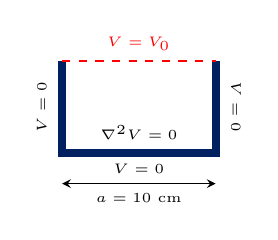
\begin{tikzpicture}[scale=0.65]
    \draw[line width=1mm, unibblue] (0,1.8) -- (0,0) -- (3.0,0) -- (3.0,1.8);
    \draw[dashed, red, thick] (0,1.8) -- (3.0,1.8) node[midway, above, font=\tiny] {$V=V_0$};
    \node at (1.5,0.4) [font=\tiny] {$\nabla^2 V = 0$};
    \node at (-0.4,0.9) [font=\tiny, rotate=90] {$V=0$};
    \node at (3.4,0.9) [font=\tiny, rotate=-90] {$V=0$};
    \node at (1.5,-0.3) [font=\tiny] {$V=0$};
    \draw[<->, >=stealth] (0,-0.6) -- (3.0,-0.6) node[midway, below, font=\tiny] {$a = 10\text{ cm}$};
  \end{tikzpicture}%
  }%
\end{minipage}\par\vspace{1mm}
\begin{answerbox}{Ruang Pengerjaan C3 (Penurunan Solusi Analitis Potensial Laplace 2D)}
  \vspace{2.8cm}
\end{answerbox}

\newpage
% ==================== HALAMAN 2 ====================

% Soal C4
\noindent\textbf{4. (C4 - Menganalisis \textbar\ Bobot: 20 Poin)}\par\vspace{0.5mm}
{\footnotesize Berdasarkan fungsi potensial $V(x,y)$, hitung komponen vektor medan listrik $E_x = -\frac{\partial V}{\partial x}$ dan $E_y = -\frac{\partial V}{\partial y}$. Analisis lokasi di mana konsentrasi stres medan listrik ($|\vec{E}|$) mencapai nilai tertinggi pada geometri tersebut.}
\begin{answerbox}{Ruang Pengerjaan C4 (Analisis Vektor Medan Listrik \& Konsentrasi Stres)}
  \vspace{3.8cm}
\end{answerbox}

\vspace{1.5mm}

% Soal C5
\noindent\textbf{5. (C5 - Mengevaluasi \textbar\ Bobot: 20 Poin)}\par\vspace{0.5mm}
{\footnotesize Evaluasi batas medan tembus korona Peek ($E_{\text{kritis}} \approx 30\text{ kV/cm}$ di udara pada kondisi atmosfer standar) pada permukaan isolator rantai 150 kV. Evaluasi efektivitas pemasangan cincin korona (\textit{corona ring}) untuk meratakan gradien potensial.}
\begin{answerbox}{Ruang Pengerjaan C5 (Evaluasi Bahaya Korona \& Efektivitas Cincin Perata)}
  \vspace{3.8cm}
\end{answerbox}

\vspace{1.5mm}

% Soal C6
\noindent\textbf{6. (C6 - Merancang \& Komputasi Julia \textbar\ Bobot: 15 Poin)}\par\vspace{0.5mm}
{\footnotesize Rancang skrip algoritma iterasi relaksasi Gauss-Seidel / SOR (\textit{Successive Over-Relaxation}) dalam bahasa \textbf{Julia} untuk menghitung matriks grid beda hingga (FDM) potensial 2D: $V_{i,j} = \frac{1}{4}(V_{i+1,j} + V_{i-1,j} + V_{i,j+1} + V_{i,j-1})$.}
\begin{answerbox}{Ruang Pengerjaan C6 (Skrip Algoritma FDM Relaksasi Gauss-Seidel Julia)}
  \vspace{3.8cm}
\end{answerbox}

\vspace{1.5mm}

% Tabel Rekapitulasi Skor OBE & Tanda Tangan
\noindent\begin{minipage}[b]{0.65\textwidth}%
  \centering
  \scriptsize
  \begin{tabular}{|c|c|c|c|c|c|c|}
    \hline
    \rowcolor{unibblue}
    \textbf{\color{white}C1} & \textbf{\color{white}C2} & \textbf{\color{white}C3} & \textbf{\color{white}C4} & \textbf{\color{white}C5} & \textbf{\color{white}C6} & \textbf{\color{white}Total} \\
    \rowcolor{unibblue!10}
    10 Pts & 15 Pts & 20 Pts & 20 Pts & 20 Pts & 15 Pts & 100 Pts \\
    \hline
    & & & & & & \\[2.5mm]
    \hline
  \end{tabular}%
\end{minipage}%
\hfill%
\begin{minipage}[b]{0.32\textwidth}%
  \centering
  \scriptsize
  \textbf{Verifikasi Dosen / Asisten:}\\[5mm]
  (\dotfill)
\end{minipage}\par

\end{document}
